

\documentclass{abstract_hutech}
\usepackage{color}
\usepackage{xcolor}
\usepackage{soul}
\usepackage[normalem]{ulem}


\newcommand{\REVIEW}[1]{\textcolor{blue}{#1}} % REVIEW is necessary later
\newcommand{\review}[1]{\textcolor{blue}{#1}} % REVIEW is necessary later
\newcommand{\FIXME}[1]{\textcolor{red}{#1}} % should be fixed later
\newcommand{\fixme}[1]{\textcolor{red}{#1}} % should be fixed later
\newcommand{\TODO}[1]{\textcolor{purple}{#1}} % TODO
\newcommand{\todo}[1]{\textcolor{purple}{#1}} % TODO
\newcommand{\eg}{\textit{e.g.,}}
\newcommand{\etal}{\textit{et al.}}
\newcommand{\ie}{\textit{i.e.,}}

\newcommand{\SJ}[1]{\textcolor{orange}{#1}} % for Sungjin
\newcommand{\CW}[1]{\textcolor{brown}{#1}} % for Chanwoo % using same color as Arvind (green hard to read..)
\newcommand{\AR}[1]{\textcolor{brown}{#1}} % for Arvind

\newcommand{\ours}{LSM-KVD}

\usepackage{hyperref}
\usepackage{subfig}
\begin{document}
\thispagestyle{firstpage}
\twocolumn[
	\begin{@twocolumnfalse}
	\vspace*{20pt}
	\begin{flushleft}
	\fontsize{20}{0}\selectfont{\textbf{LSMKVD: Log Structured Merge tree Key-Value Drive}}
	\vspace{32pt}\par
	\fontsize{10}{12}\selectfont{\textbf{(Abstract) This is a template of Extended Abstract for HumanTech Paper Award. The recommended volume is 2 pages with 2-column format. Titles do not exceed two lines and abstracts do not exceed 15 lines.\\
		Papers should be written in Times New Roman font with the font size of 20pt in bold for the title, 10pt in bold for abstracts, 11pt in bold for the titles within text, 10pt for the text, 9pt in bold for the titles of figures and tables and 9pt for the references. For the fairness of the review, Name, major, the school/university name, the school/university logo, and teacher/professors name of author should not be included in the abstract and paper.
	}}
\end{flushleft}
\vspace{20pt}
\end{@twocolumnfalse}
]

\section{INTRODUCTION}
Key-Value store (KVS) has become a necessary infrastructure for many applications, such as caching, web indexing, and storage systems~\cite{memcached,tao,bigtable,dynamo}.  
Owing to its popularity and huge impact on application performance, serious efforts have been made to optimize KVS at various levels: algorithm~\cite{silk,dostoevsky,monkey,blsm},
system~\cite{wisckey,wang2014efficient,flashstore}, and architecture~\cite{bluecache,kvs-fpga1,kvs-fpga2}.

Another approach is to offload most of the key-value (KV) functionality onto a storage device, the so-called KV-SSD~\cite{kvssd,kaml,nvmkv,bluecache}.  
By making the storage hardware directly serve KV requests via a driver, KV-SSDs enable clients to bypass the deep software stack in the host.
For example, by performing most commonly used operations of KV databases, such as RocksDB~\cite{rocksdb}, 
%file systems, and block I/O subsystems are no longer needed.
in KV-SSDs, we not only improve I/O latency and throughput of the operations but also reduce host resources \textcolor{red}{CPU and Memory}.
%But The idea of KV-SSD is promising but the current proposals and products often provide inconsistent tail latency and throughput degradation.
%Because of those KV-SSDs are based on Hash.

The existing ideas using hash algorithm for managing KV pairs because it has a simple architecture -- it maintains a hash table in the controller DRAM.
However, if the DRAM size is not large enough to hold all the hash entries, parts of the hash table must be stored in flash.
%(\ie{} in-flash hash table). 
This inevitably involves expensive flash accesses to look for a key when it is not found in the DRAM-resident hash table.  
Even worse, if a hash collision occurs then multiple flash accesses may be required, resulting in long tail latency and drop in throughput.

An alternative to hashing is a \emph{log-structured merge tree} (LSM-tree)~\cite{lsm-tree}. which can provide stable read latency by the level structure and write throughput.
However, it offers bad average read performance. Also Compaction, an essential requirement of LSM-tree implementation, is problematic because it requires sorting~\cite{wisckey,blsm,silk}.
CPU cycles for sorting can become a huge burden on embedded CPUs in SSD controllers. Extra I/O operations to keep KV pairs sorted further deteriorate I/O throughput.  
Due to these drawbacks, LSM-tree has not been considered an attractive solution for KV-SSDs.

In this paper, we show that, by optimizing the LSM-tree algorithm and tightly integrating it with an SSD controller, LSM-tree-based KV-SSDs can outperform hash-based designs.  
Our solution is based on three ideas.
First, pin all KV indices of the top levels of the tree to DRAM to speedup reads.
This level pinning not only guarantees the worst-case read latency, but improves average latency by reducing flash look-ups for retrieving KV indices.  
Second, run sorting tasks using HW accelerators, in parallel with I/O tasks to eliminate CPU overheads for compaction.
Third, combine level-pinning with key-value separation~\cite{wisckey} to reduce I/O overheads for compaction.
Collectively these techniques remove the compaction bottleneck and provide high write-throughput.
We believe that our techniques can also be applied profitably to general LSM-tree implementations, which may not have the same resource constraints as KV-SSDs do.

Based on these ideas, we have designed a new LSM-tree-based KV-SSD, called
\textit{\ours{}} and implemented it on an FPGA-based SSD
platform~\cite{bluedbm}. Using micro and YCSB~\cite{ycsb} benchmarks, we have
shown that \ours{} outperforms existing KV-SSD designs in \textcolor{red}{XX to XX on IOPS, YY on tail latency},
%including tail read-latency, average read-latency, and I/O throughput.  It is
%well known that the LSM-tree algorithm offers an intrinsic tradeoff between
%read-latency and write-throughput, controlled by the tree height~\cite{dostoevsky,monkey}.  We have quantified this tradeoff and shown that for
%a given DRAM capacity an application can configure our implementation to
%support its KV performance requirements.  Alternatively, the manufacturer can
%supply more DRAM to support KV applications requiring higher performance.
%For example, for a write-intensive workload, \ours{} improves throughput by
%31\% by sacrificing average read latency by 7.4\% but with guaranteed tails.

\section{MOTIVATION}


\subsection{Problems of Hash-based Design}
\label{sec:hash-kvssd:problem}
A hash-based KV-SSD maintains a hash table with many buckets in the controller DRAM, where each bucket holds metadata, \ie{} a key and a pointer, for a specific KV object in flash~\cite{nvmkv,flashstore,bluecache,kaml}.  
The \texttt{SET(),GET()} operations on a KV object first calculates a bucket index  using a hash function, \ie{} \texttt{index} = \texttt{hash(key)}.
This simple architecture offers fast response time for both operations. This simplicity and efficiency,
however, assume that the SSD has a large enough DRAM in its controller to hold
all the hash buckets.  In practice, product SSDs do not have enough DRAM.
Suppose that the SSD capacity is 4 TB and it has 4 GB DRAM is available for
indexing.  Further suppose the key and value sizes are on average 32 B and 1
KB, respectively~\cite{kvsize}.  If the number of buckets is $2^{32}$ (=
$2^{42}/2^{10}$) and the bucket size is 36 B (32 B for key and 4 B for
pointer), we will need 144 GB of DRAM to hold the complete hash table!
also using signature (16 bits)~\cite{kvsdd} instead of key can't overcome the problem. it needs 24GB memory in same setting. 

To run KV-SSD with limited DRAM, we can borrow an idea from demand-based FTLs~\cite{dftl} which keep only popular buckets in DRAM, while storing the rest in the flash.
This, however, causes extra flash reads while retrieving KV objects. 
If a designated bucket is not available in DRAM (\ie~\textit{hash-table miss}), 
we have to fetch the bucket from the flash first to
find the location of a desired KV object.



\subsection{Experiments with Product KV-SSD}
\label{sec:hash-kvssd:exp}

\begin{figure}[t]
    \centering
    \subfloat[CDF of read latency (KV-SSD)]{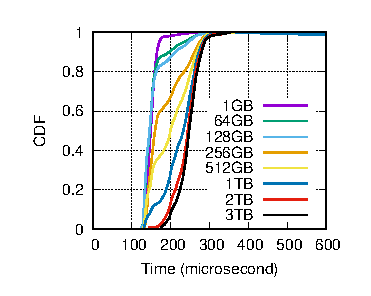
\includegraphics[width=0.24\textwidth]{exp/kvssd_latency_iops/kvssd_latency/kvssd_rlatency_trend.eps}} 
    \subfloat[CDF of read latency (KV-SSD)]{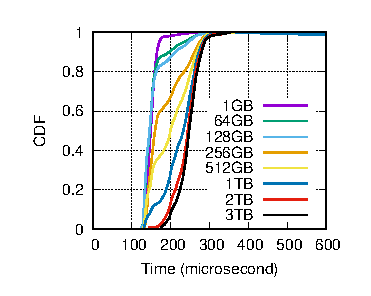
\includegraphics[width=0.24\textwidth]{exp/kvssd_latency_iops/kvssd_latency/kvssd_rlatency_trend.eps}}
%   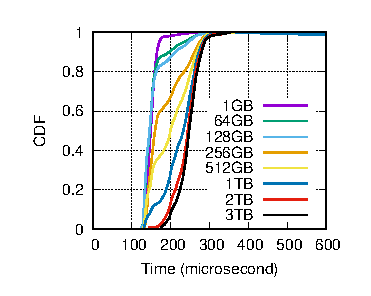
\includegraphics[width=0.24\textwidth]{exp/kvssd_latency_iops/kvssd_latency/kvssd_rlatency_trend.eps}
    \caption{Experimental results with Block-SSD and KV-SSD}
    \label{fig:hash-kvssd-exp}\vspace{-13pt}
\end{figure}
To confirm our analysis, we carried out experiments using a KV-SSD product
(3.84~TB PM983~\cite{pm983,kv-pm983}). The internal architecture of the
KV-SSD model is not disclosed to the public, except that it is based on
hash-based data structures~\cite{kvssd}.

\textbf{Experimental Setup:}
The number of KV objects stored in a KV-SSD  directly affects its performance. 
This is because, as the number of KV objects increases, more memory is required for the hash-map, which may result in frequent signature collision and/or hash-map misses.  
Based on this fact, we conduct experiments in two phases: \textit{load} and \textit{run}. 

The load phase creates an object pool on an empty SSD by writing a bulk of KV objects.
The default key and value sizes were 16 B and 1 KB, respectively.
Various sizes of object pools, from 1 GB to 3 TB, were created. 
For example, a 1GB-pool contained 1M KV objects.
During the run phase, we executed KVBench~\cite{kvbench} on the object pools.
KVBench generated random \texttt{GET} requests and ran for 10 minutes. 
We measured read latency and throughput.
When measuring read latency, the queue depth (QD) was set to 1
to eliminate noises from queueing delays. To measure the maximum throughput the
KV-SSD can achieve, QD was set to 64.

\textbf{Result:}
% Block-SSD average = 110 usec and consistent 
Figures~\ref{fig:hash-kvssd-exp}(b) and (c) shows the read latency and
throughput of the KV-SSD.  The KV-SSD showed inconsistent read response times
as the number of objects stored got larger.  In particular, the average read
latency increased  from 149.49 $\mu$s to 245.31 $\mu$s (1.64X), when the object
pool-size was increased from 1~GB to 3~TB.  We also observed very long tail
latency.  For the 99.99th percentile, the KV-SSD tail latency increased from
323 $\mu$s to 1020 $\mu$s when object pool was increased from 1 TB to 3 TB.
Even worse, as depicted in Figure~\ref{fig:hash-kvssd-exp}(c), the read
throughput continued to drop as the object pool size got larger, for example,
from 112 KIOPS to 64 KIOPS.

\section{\ours{}}
\begin{figure}[h]
	\centering
	%\subfloat[layout]{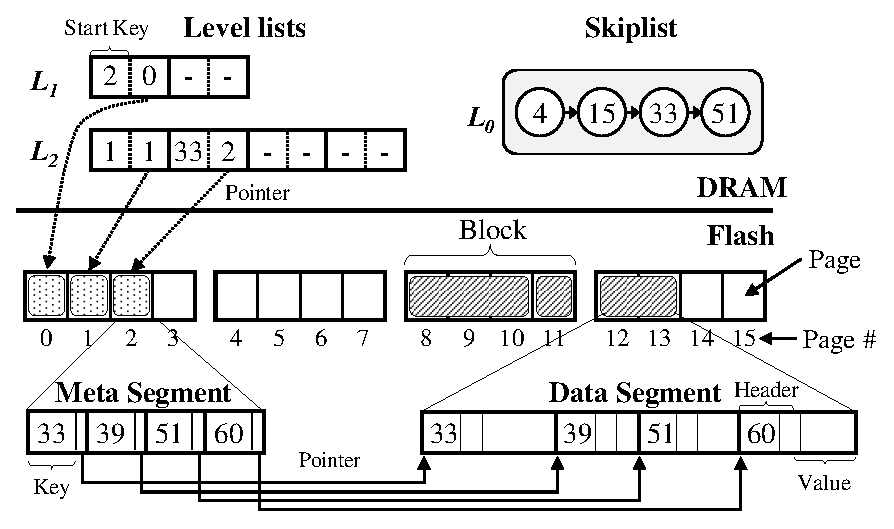
\includegraphics[width=0.24\textwidth]{fig/fig3.eps}}
	%\subfloat[Flush & Compaction]{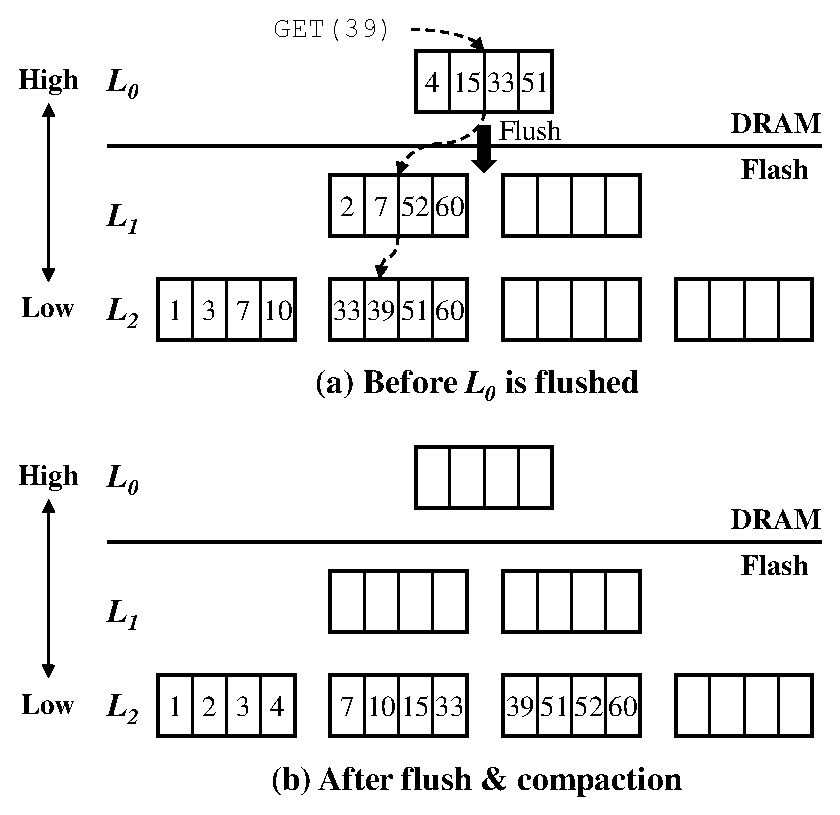
\includegraphics[width=0.24\textwidth]{fig/fig1.eps}}
	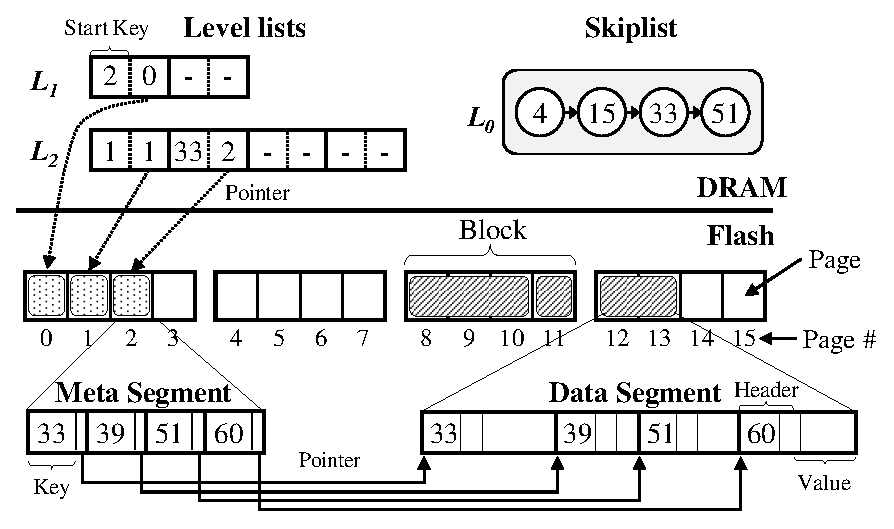
\includegraphics[height=4.5cm]{fig/fig3.eps}
	\caption{LSMKVD Layout}
	\label{fig:overall}\vspace{-11pt}
\end{figure}

\subsection{Design of \ours{}}
\ours{} has four types of data structures to implement the LSM-tree algorithm
(Figure~\ref{fig:overall}): a \textit{skiplist} and \textit{level lists}, which
all reside in DRAM, and  \textit{meta segments} and \textit{data segments},
which all reside in flash.  We describe how these data structures are
managed and then estimate its DRAM requirement. 

The skiplist corresponds to $L_0$ in the LSM-tree algorithm, and holds 64 MB of KV
objects which is large enough to fully utilize the parallelism of a NAND chip
array.  Each skiplist entry has four fields: <key size, key, value size,
value>, and the skiplist is kept sorted by the keys. 

In our design, each meta segment belongs to one of the levels in the tree.
\ours{} maintains another in-memory data structure, \textit{level lists}, which
keeps track of meta segments at every level in the flash.  Each level list is
an array of pointers (4 B each) to meta segments belonging to the level.  Each array
entry also contains the start key (a variable size from 16 B to 128 B) of the meta segment to facilitate searching.
Figure~\ref{fig:overall} illustrates examples of how the level lists point to
meta segments which, in turn, point to actual values.

\textbf{DRAM Requirement for Level Lists:}
Let's estimate DRAM requirement of~\ours{}.  We assume that an
SSD capacity is 4 TB and each meta segment is 32 KB. First 
consider the case where the average sizes of keys and values are 32 B and 1 KB,
respectively~\cite{kvsize}. In this case only 162 MB DRAM is needed to hold all the level lists.
For the
worst-case scenario, where all the objects have the maximum key size of 128 B,
the level lists would require about 2.1 GB DRAM.  This can still easily fit in
4 GB DRAM that 4 TB SSD has for mapping.

\subsection{Optimizing Technics}
\textbf{Optimizing read Latency:}
Retrieving a KV object from \ours{} requires multiple flash lookups. 
\ours{} first looks up the
skiplist ($L_0$). If a matched one is not found, it has to go down to
$L_1$. \ours{} looks up the $L_1$ level list to get the location of a meta
segment that \textit{may} have an index for a desired KV object. If $L_1$ doesn't have the target key mapping, it is going down to the next level. Finally at most N (\# of Levels) look up is needed for getting a KV objects.

To reduce these look up costs, \ours{} adopts aggressive strategy: \textit{level pinning}.  If the LSM-tree has $n$
levels, \ours{} keeps meta segments for top-$k$ levels ($k \le n-1$) in DRAM.
To process a \texttt{GET} request, it first searches for a key in top-$k$
levels in DRAM.  Only when a key is not found there, it lookups the rest
of levels resident in the flash.  With the level pinning, the number of the
worst-case flash lookups is reduced to $O(n-k-1)$. 

\textbf{Optimizing compaction:}
To keep each level sorted, \ours{} performs compaction which involves extra I/Os and CPU cycles.
By using \textit{level pinning} techning and seperating keys from values{~\cite{wisckey}}, it can reduce I/O traffics in compaction phase. 
However, The sorting overhead of compaction is pretty huge on embedded system. 
We address this problem by offloading sorting tasks to a special hardware accelerator in the SSD controller. It can reduce CPU times \todo{XX to YY} which is almost 0.

\subsection{Memory and Performance Trade-offs}

\section{EXPERIMENTS}
\subsection{Experimental Setup}
We implemented the \ours{} software and hardware accelerator on our FPGA-based
SSD platform that has a quad-core ARM Cortex-A53 CPU running at 1.2 GHz with 16 GB
DRAM. This hardware specification is almost equivalent to those of recent SSDs.

For realistic experiments, We implemented the hash-based KVSSD using 8 bits signature. It makes more entries caching.
And \ours{} is pinning top 3 levels among the total 5 levels.
To confirm effect of the HW-accelerator, We tested two diffrent versions of \ours.
One is \texttt{LSM-KVD}, another is \texttt{LSM-KVD+} which adopt the HW-accelerator.

\subsection{YCSB}
We measured IOPS and read latency of the hash-based KV-SSDs and \ours{} while running YCSB.
\todo{explanation of A,C,D,E workloads}.

\begin{figure}[h]
\centering
\includegraphics[width=3.4cm,angle=-90]{./exp/exp1/exp1.eps}
\caption{
Throughput comparison of KV-SSD and \ours{}
}
\label{fig:iops}
\vspace{-10pt}
\end{figure}
\textbf{IOPS:}
\ours{} outperformed the
hash-based ones, providing 47\% higher IOPS, on average. Particularly, for
YCSB-E with range queries, \ours{} showed 71$\sim$111\% higher IOPS thanks to
LSM-tree's sorted nature. 

In case of YCSB-C, Because \ours{} doesn't have any cache mechanism, It is weak when the workload has read after read the same key. 
But In case of YCSB-D, otherwise, it performed very well because the workload's pattern is read after write same key. Almost keys were hitted in level pinning.

And thanks to the HW-accelerator, \texttt{LSM-KVD+} has better performanc than \texttt{LSM-KVD} on all workloads including \texttt{SET} operation.
\begin{figure}[h]
\centering
\includegraphics[height=0.5\textwidth,angle=-90]{./exp/exp2/exp2.eps}
\caption{
CDF graphs of read latency of the hash-based KV-SSD and \ours{}
}
\label{fig:cdf}
\vspace{-10pt}
\end{figure}

\textbf{Read Latency:}
Figure~\ref{fig:cdf} shows CDF graphs of read response times of all three types of KVSSD from 95\% to 99.99\%.

\texttt{Hash} was suffer collision on all workloads. 
However, By using level pinning \ours{} can guarantee that \texttt{GET} can be done in two flash lookups.
Thus, \ours{} beat \texttt{Hash} on all workloads.

\begin{thebibliography}{99}

\end{thebibliography}

%\bibliographystyle{acm}
%\bibliography{references}
\end{document}
